% =============================================================================
\section{Introduction}
% =============================================================================
The processing in WSN applications is often intimately tied to the
environment the system is immersed in. Consider for example a health
monitoring application~\cite{ko10wireless}, whose goal is to
continuously monitor an individual's physical conditions. Body-worn
sensors track quantities such as heart rate and body movements. In
normal conditions, the monitoring rate may be limited to save
energy. Whenever a potentially harmful condition is detected, the
sensors increase the monitoring rate to obtain finer-grained
information. Orthogonal to application-level functionality, the system
should periodically transmit sensed data to a back-end whenever a
network infrastructure is in reach, such a residential Internet
gateway, or locally log data in infrastructure-less situations.

% smart home application, whose goal is to improve the user comfort
% while saving energy due to heating or air conditioning. Environmental
% sensors are deployed in every room to monitor temperature and
% humidity. Body-worn sensors track the inhabitants location in the
% house. Based on these information, the system decides how to tune air
% conditioning in every room depending on current conditions and usage
% patterns.
 
Designing and implementing similar applications is currently
intricate. The number of possible different situations that developers
must account for may be prohibitively large. The problem is often
exacerbated by the interplay between application-level and
system-level functionality, which may often be a function of
independent environmental quantities, as in our example health
monitoring application. As a result, implementations become entangled
and thus difficult to re-use, to debug, and to maintain.

% Indeed, the processing aboard WSN nodes becomes a function
% of the surrounding environmental conditions. For example, an
% environmental node recording temperature and humidity conditions
% within the user tolerance may refrain from reporting further data to
% where the actuation decisions are taken. Should the node detect high
% temperature conditions, a notification to trigger air conditioning is
% to be generated in case body-worn sensors detect a person in the same
% room. % Addressing similar requirements often leads to very complex
% % source code.

% Wireless Sensor Networks (WSNs) can be applied in different areas \cite{pastor08}. In this paper we use Smart Home as a particular example. This application of WSN have to track householder location and execute a list of instructions depending on it. In parallel, WSN should monitor and control a climate in the house. On the hardware level WSN have sensors to monitor the environment (like temperature, light intensity etc.), which are static. There are also mobile sensors, which are attached to the householder to track his location inside and outside the house. In order to ensure an appropriate quality of service, they should provide a long work time and be as autonomous as possible. These requirements lead to very complex source code. To reduce the complexity we propose to use Context-Oriented paradigm.

\marginpar{
  \begin{figure}
    \centering
    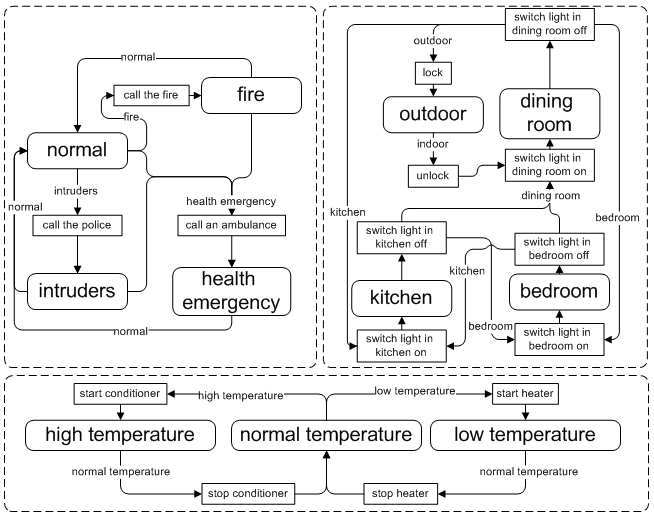
\includegraphics[width=\marginparwidth]{smarthome.png}
    \caption{Context diagram for Smart Home WSN.}
    \label{fig:cdsm}
  \end{figure}
}

We argue that promoting a notion of \emph{context} as a first-class
citizen in WSN programming facilitates the design and implementation
of environment-dependent functionality. Context here indicates ``any
information that can be used to characterize the situation of an
entity, where an entity can be a person, place, or physical object"
\cite{dey99}. In this work, we leverage concepts of Context-Oriented
Programming (COP)~\cite{hirschfeld08} to support programmers in
developing software that can dynamically change its behavior depending
on context
information. % Using context as a building block, programmers can more
% effectively craft WSN applications that are aware of changes in the
% environment.

% Thus, COP could be used as an effective way to use a \textit{Context} for developing a software for WSNs. It also will help to avoid the increasing complexity of a program. In our example (Smart Home) there are a lot of possible \textit{contexts}, which are depending on the type of sensor, state of the environment and location of the householder. Some of \textit{contexts} are mutually exclusive, while other can be activated in parallel. For example, usually householder can not move from bathroom directly outside the house, thus this kind of the location change should be treated as an error. But climate state does not depend on the householder's location and corresponding \textit{contexts} can be activated or deactivated independently.

Applying COP to WSNs programming is, however, accompanied by several challenges:
\begin{itemize}\compresslist
\item As our health-care application demonstrates, in WSNs
  different context information can have complex interactions and
  interconnections; it is then necessary to use custom abstractions
  and expressly tailored programming techniques.
\item Traditional WSN programming languages favor static memory
  management and lack features such as object-orientation and dynamic
  programming; therefore, COP approaches designed for high-level
  languages like Java or Python are not applicable.
\item WSN platforms feature constrained hardware resources, such as
  small amounts of memory, limited computation facilities, and power
  consumption constraints; the solutions to the challenges above must
  thus live with such limitations.
\end{itemize}

We describe next how we meet these challenges. At the core of our
solution is a dedicated programming model and language called
{\textlst{ConesC}}. The latter extends the nesC~\cite{gay03:nesc}
language for sensor networks with COP constructs. Particularly, we
enable a notion of \emph{layered function}~\cite{hirschfeld08} in
nesC. Programmers provide different implementations of the \emph{same}
layered function that specify different behaviors depending on context
information. The system then automatically dispatches function calls
to the ``right'' implementation, that is, the one associated with the
currently perceived context. This greatly simplifies implementing
context-dependent functionality, rendering code
simpler to read, to maintain, and to debug.


%%% Local Variables: 
%%% mode: latex
%%% TeX-master: "ubicomp"
%%% End: 
